%
% Tutorial -- Lineal blocks and frequency response
% Copyright (C) 2019 Romano Giannetti <romano.giannetti@gmail.com>
%
% This is free software; you can redistribute it and/or modify
% it under the terms of the GNU General Public License as published by
% the Free Software Foundation; either version 2, or (at your option)
% any later version.
%
% This software is distributed in the hope that it will be useful,
% but WITHOUT ANY WARRANTY; without even the implied warranty of
% MERCHANTABILITY or FITNESS FOR A PARTICULAR PURPOSE.  See the
% GNU General Public License for more details.
%
% You should have received a copy of the GNU General Public License
% along with this package; see the file COPYING.  If not, write to
% the Free Software Foundation, Inc., 51 Franklin Street - Fifth Floor,
% Boston, MA 02110-1301, USA.%
%        File: ampli_qucs_tut.tex
%     Created: Fri Jan 24 05:00 PM 2014 M
% Last Change: Fri Jan 24 05:00 PM 2014 M
% Submitted:   Sun Feb 3 08:00 PM 2019 CET
%
% \documentclass[a4paper,12pt]{article}
% \usepackage{graphicx}
% \usepackage[margin=2cm]{geometry}
%% my parameters for formatting
% \parindent=0pt
% \parskip=6pt plus 6pt minus 3pt\relax
%% my macros
\documentclass[12pt,a4paper,oneside]{report}

% Include basic and title page definitions.
%
% This document contains a generic preamble for tutorials.
%
% Copyright (C) 2005 Stefan Jahn <stefan@lkcc.org>
%
% Permission is granted to copy, distribute and/or modify this document
% under the terms of the GNU Free Documentation License, Version 1.1
% or any later version published by the Free Software Foundation.
%

% Load some packages.
\newcommand{\tutpackages}{%
  \usepackage{savesym}
  \usepackage{geometry}
  \usepackage[T1]{fontenc}
  \usepackage{longtable}
  \usepackage{ae,aecompl}
  \usepackage{url}
  \usepackage{epsfig}
  \usepackage{array}
  \usepackage{subfigure}
  \usepackage{amsmath}
  \usepackage{amsfonts}
  \usepackage{verbatim}
  \usepackage{fancyvrb}
  \savesymbol{iint}
  \usepackage{stmaryrd}
  \usepackage{wasysym}
  \restoresymbol{WASY}{iint}
  \usepackage{pifont}
  \usepackage[amssymb]{SIunits}
  \usepackage{graphics}
  \usepackage{psfrag}
  \usepackage{relsize}
  \usepackage[section]{placeins}
  \usepackage{listings}
  \usepackage{tikz}
  \usepackage{amssymb}
  \usepackage{amsmath}
  \iftutbook
  \else
    \usepackage{makeidx}
    \makeindex
  \fi
}

% Compatibility code for LaTeX and pdfTeX.
\newcommand{\tutcompat}{%
  \newif\ifpdf
  \ifx\pdfoutput\undefined
    \pdffalse
  \else
    \pdfoutput=1
    \pdftrue
  \fi
}

% Only evaluated if run using pdfTeX.
\newcommand{\tutheader}[2]{%
  \ifpdf
    \usepackage[pdftex,
	a4paper,
	backref,
	\iftutbook
	  anchorcolor=black,
	  filecolor=black,
	  menucolor=black,
	  pagecolor=black,
	  bookmarks=true,
	  bookmarksopen=true,
	  bookmarksnumbered=true,
	  pdfpagemode=UseOutlines,
	\else
	  bookmarks=false,
	  bookmarksopen=false,
	  bookmarksnumbered=true,
	  pdfpagemode=UseNone,
	\fi
	baseurl={http://qucs.sourceforge.net},
	pdfstartview=FitH,
	pdftitle={Qucs - \tuttitle},
	pdfauthor={#2},
	pdfsubject={#1},
	colorlinks,
	linkcolor=black,
	urlcolor=black,
	citecolor=black,
	backref=false,
	plainpages=false,
	pagebackref=false]{hyperref}
    \DeclareGraphicsExtensions{.pdf,.png}
    \pdfcompresslevel 9
    \pdfinfo {
      /Title   (Qucs - \tuttitle)
      /Subject (#1)
      /Author  (#2)
    }
  \else
    \DeclareGraphicsExtensions{.eps}
  \fi
  \graphicspath{{pics/}}
}

% Generic tutorial startup code.
\newcommand{\tutstartup}[2]{%
  \tutpackages
  \tutcompat
  \tutheader{#1}{#2}
}

% Begin document.
\newcommand{\tutbegin}{%
  \begin{document}
  \tuttitlepage
  \setlength{\parindent}{0pt}
}

% End document.
\newcommand{\tutend}{%
  \end{document}
}

\include{titlepage}

\tuttitle{
  A Tutorial}
\tutsubtitle{
  Linear blocks and frequency response}
\tutauthor{
  Romano Giannetti}
\tutcopyright{
  Copyright \copyright{} 2019 Romano Giannetti
  \textless romano.giannetti@gmail.com\textgreater\\
  }
\tutbookfalse

\tutstartup{\tutsubtitle}{Romano Giannetti}

\tutbegin

\makeatletter
\def\fname#1{%
  \edef\@tempa{#1}%
   \texttt{\expandafter\strip@prefix\meaning\@tempa}}%
\makeatother
%
\newcommand{\button}[1]{``#1''}
\newcommand{\component}[1]{``#1''}
\newcommand{\tab}[1]{\textsl{#1}}
\newcommand{\menu}[1]{\texttt{#1}}
\newcommand{\dropdown}[1]{\texttt{#1}}
\newcommand{\key}[1]{\texttt{<#1>}}
\newcommand{\var}[1]{\textsf{#1}}

\newcommand{\screenshot}[1]{\par\smallskip
  \includegraphics[width=0.7\textwidth]{#1}\par\smallskip}
\newcommand{\twoscreenshot}[2]{\par\smallskip
  \includegraphics[width=0.475\textwidth]{#1}\quad
  \includegraphics[width=0.475\textwidth]{#2}\par\smallskip}

% \begin{document}
% \title{A gentle introduction to Qucs:\\ simulating a linear circuit}
% \author{Romano Giannetti, \fname{romano.giannetti@gmail.com}}
% \maketitle

\tutsection{Presenting the Problem}

This is a step by step tutorial on how to use Qucs to simulate multi-stage amplifier (with very simple and basic approach).
It is thought to show a couple of interesting things of Qucs and to get started with the program basics.

Suppose you have to study the effect of the variation of the input impedance of the first  of the two amplifier stages on amplification and bandwidth in the following circuit.

\begin{center}
  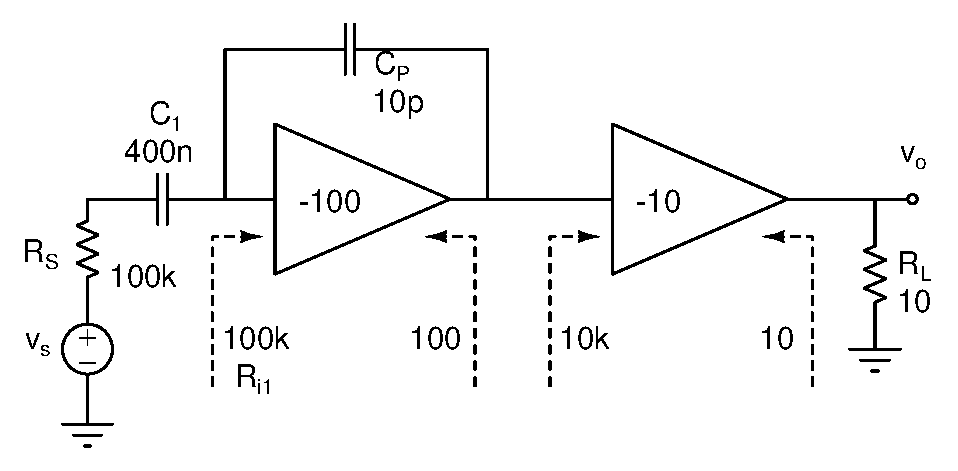
\includegraphics[width=0.7\textwidth]{theproblem}
\end{center}

\tutsection{Defining our amplifier block}

Let's start with defining a new project (\fname{ampliBW}) and creating a schematic for it.
Use \button{New} from the \tab{Projects} tab on the left pane; choose a name and then press \button{Create}.

\screenshot{step001}

Then we have to create a schematic for our simulation.
Let's create one and then put in the source generator.
Go to the \tab{untitled} tab you have at the right and choose \menu{File, Save as\ldots,} and then choose a name, like \fname{main_circ.sch}.

\screenshot{step002}

Ok, now you have your canvas where to draw your circuit.
Let's start with the generator. We want to perform a frequency domain analysis, so we need a sinusoidal generator to start with.
The components for our circuit are found in the \tab{Components} tab (surprisingly!), where you have to choose the categories using the upper drop-down.
So you will find the resistance in \dropdown{lumped components} and the generator under \dropdown{sources}.
Simply select the componet and move it to the canvas.
You can then rotate them and wire them together with the rotate and the wire tool.
Ground is conveniently available in the main bar.

\twoscreenshot{step003}{step004}

Now let's edit the component values. Right-click on the resistor (with the arrow selected --- you can get there from the other tools by pressing \key{Esc}) and edit the values you want; in this case the value of the resistor.
Remember to press \key{Enter} at the end, or Qucs will not honor your change.


\twoscreenshot{step005}{step006}

Now we have to put the amplifier in. Let's define a \emph{subcircuit} to represent it: so that we can reuse it in the circuit multiple times.

To build a subcircuit, you need to create  a new subcircuit sheet, and draw another schematics --- so go in \tab{Content}, choose \menu{File, New}, and the again \menu{File, Save as\ldots} and use for example the name \fname{ampli_v}. You will have the following screenshot:


\screenshot{step007}

Now let's draw our equivalent circuit. The trick to make it a subcircuit is to put into it the special component \component{Subcircuit port} that you can find in \dropdown{lumped component}.
Our model is a two-port amplifier, so we will have four ports.
In the following two screens, notice that when you drag the ports into the circuit you can see that the system marks the circuit as a subcomponent by adding the note ``4-port'' to the \tab{Content} when you save it. After that, I added the circuit, changed the name of the ports, flipped/rotated component, and saved.

\twoscreenshot{step008}{step009}

Now we want to transform this circuit in a generic component, so we will define the values of the componets as generic variables.
This is done by editing the component and putting simbolic names to the value of the component.
In our case, we have $R_\mathit{in}$, $R_\mathit{out}$, $A_v$.

\screenshot{step010}

After that, you have to declare the parameters. Choose \menu{File, Edit Circuit Symbol} (forget for the moment what appears) and double click on the name of the subcircuit (by default \texttt{SUB}).
Edit the name of the subcircuit to your taste and add the three parameters.
Take care in using the same exact names of the previous step.

\twoscreenshot{step011}{step012}

You will have something like that during the process and at the end.

\twoscreenshot{step013}{step014}

Now let's edit the symbol so that it is less crowded. What I normal do is to spread out all the various terminals, and then work with the shapes at the left to draw something that I like (this is not the easiest interface, really, but well\ldots)

\twoscreenshot{step015}{step016}

Note some nice trick in the second (final) shot:

\begin{itemize}
  \item you can ``flip'' the symbols (especially the pins, so that you can keep the labels out of the way) with the tool marked by the number 1;
  \item you need to put label with the ``text'' tool, because the labels of the pins will not be visible by default in the main diagram;
  \item to obtain the subscript notation, you have to you a sort-of \LaTeX\ style: write \verb|\in_{ref}| to have $\mathrm{in}_\mathrm{ref}$.
\end{itemize}

\tutsection{Using the subcircuit}

Now you can go back to the main diagram. Show the ``Content'' tab in the left box, and click on the subcircuit name so that it is highlighted.
When you return with the mouse in the drawing area, the shape of your subcircuit is shown, and you can position it (various copies of it, if needed) wherever you like.

\screenshot{step017}

Proceed to add the other components and to set the value of all the components as specified in the problem. You should end with something like the following:

\screenshot{step018}

Note that I have changed all the names of the components to match the original problem, and that I have added (with the tool ``name'', marked by the arrows) the name to the input (\var{vs}) and output  (\var{vo}) nodes.

Save your work (in the main menu: \menu{File, Save All}); now we are ready to simulate.

In Qucs, to simulate you have to add the special component ``simulation'' to the circuit.
Since we want to simulate the frequency response of the of the system, and we want to plot the $v_o$ magnitude in decibel, we need two things:

\begin{itemize}
  \item An ``AC'' simulation block (this is a linear simulation with a frequency sweep, exactly what we need), and
  \item an ``Equation'' block, to calculate the module of the output voltage in dB.
\end{itemize}

Let's start with the simulation. In the components tab, choose the AC simulation and position a simulation box in the schematic.
Then choose the arrow tool again, double click on the box and edit the parameters to match your needs.


\twoscreenshot{step019}{step020}

Now you can simulate the circuit --- we still cannot have our diagram in dB, but we can start checking the correctness of the circuit used.
Press \key{F2} (or \menu{Simulation, Simulate} in the menu).

If there are no errors, Qucs will switch to a blank tab --- we should now choose what we want to display.

Select the tab \tab{Components}, dropdown \dropdown{diagrams}; pick ``cartesian'' and put it in the window. Automatically a configuration dialog will appear, with all the variables that you can plot.

\twoscreenshot{step021}{step022}

Let's choose \var{vo.v} --- as you can see, is part of the dataset with the name corresponding to your circuit, and is \var{dep}endent on \var{acfrequency}, which is the vector generated by your simulation sweep. Then choose --- we will refine that later --- a double logarithmic scale and press OK.
You will have a graph that, after a bit of resizing, will be similar to this one:

\screenshot{step023}

Now we will try to have the output graph representing the gain in dB; while at it we can change the frequency range a bit to see better the low frequencies.
To draw a variable which is not directly available, we have to define it somewhere: this is the task for ``equation''.
Insert an equation and edit it; the formula for our gain will be \var{A=20*log10(abs(vo.v)/abs(vs.v))} --- the name of the variables is the same as you saw in the graph properties dialog.

\screenshot{step024}

As you can notice, the frequency range has been changed too.
Re-run the simulation (\key{F2}) again; Qucs will switch to the graph editing properties.
Double click on the graph and change the variable to be drawn to \var{A}, and unset the tick on the log scale for the y axis.
You should now have something like that:

\screenshot{step025}

\tutsection{Parameter sweep}

Next step is to add a so-called ``parameter sweep'' to change the input resistance of the first amplifier and see what happens.

So let's start by adding a \component{SWP} from the \component{simulations} to our main circuit.

\screenshot{step026}

In the previous shot, you see that we have added a sweep parameter that

\begin{itemize}
  \item will change and repeat the simulation \var{AC1};
  \item will create a parameter named \var{Rin1},
  \item which will change in logarithmic way from 1k to 1M in 4 steps (assuming the values 1k, 10k, 100k and 1M).
\end{itemize}

Now let's use the parameter: double click on the first amplifier in the chain and change the input resistance value to the variable \var{Rin1}.

Simulate again and\ldots

\twoscreenshot{step027}{step028}

Let's add a final touch to the graph. Using the ``mark'' tool, we can add markings to each one of the lines of the graph and so see for which parameter each one has been computed.

\screenshot{step029}

(I do not know if there is a way to have each line colored different and adding a legend. Anyway, I normally export the dataset and make my graphs with \fname{pyxplot} or \fname{gnuplot}.)

As a nice icing on the cake, you can arrange the output graph and the circuit in various way, even in the same page. After that, exporting the figure in Encapsulated Postscript (form Qucs 0.0.18 only) will result in a very nice, high quality figure as the one in the following page.

\vfill\eject

\null\vfill
\begin{center}
    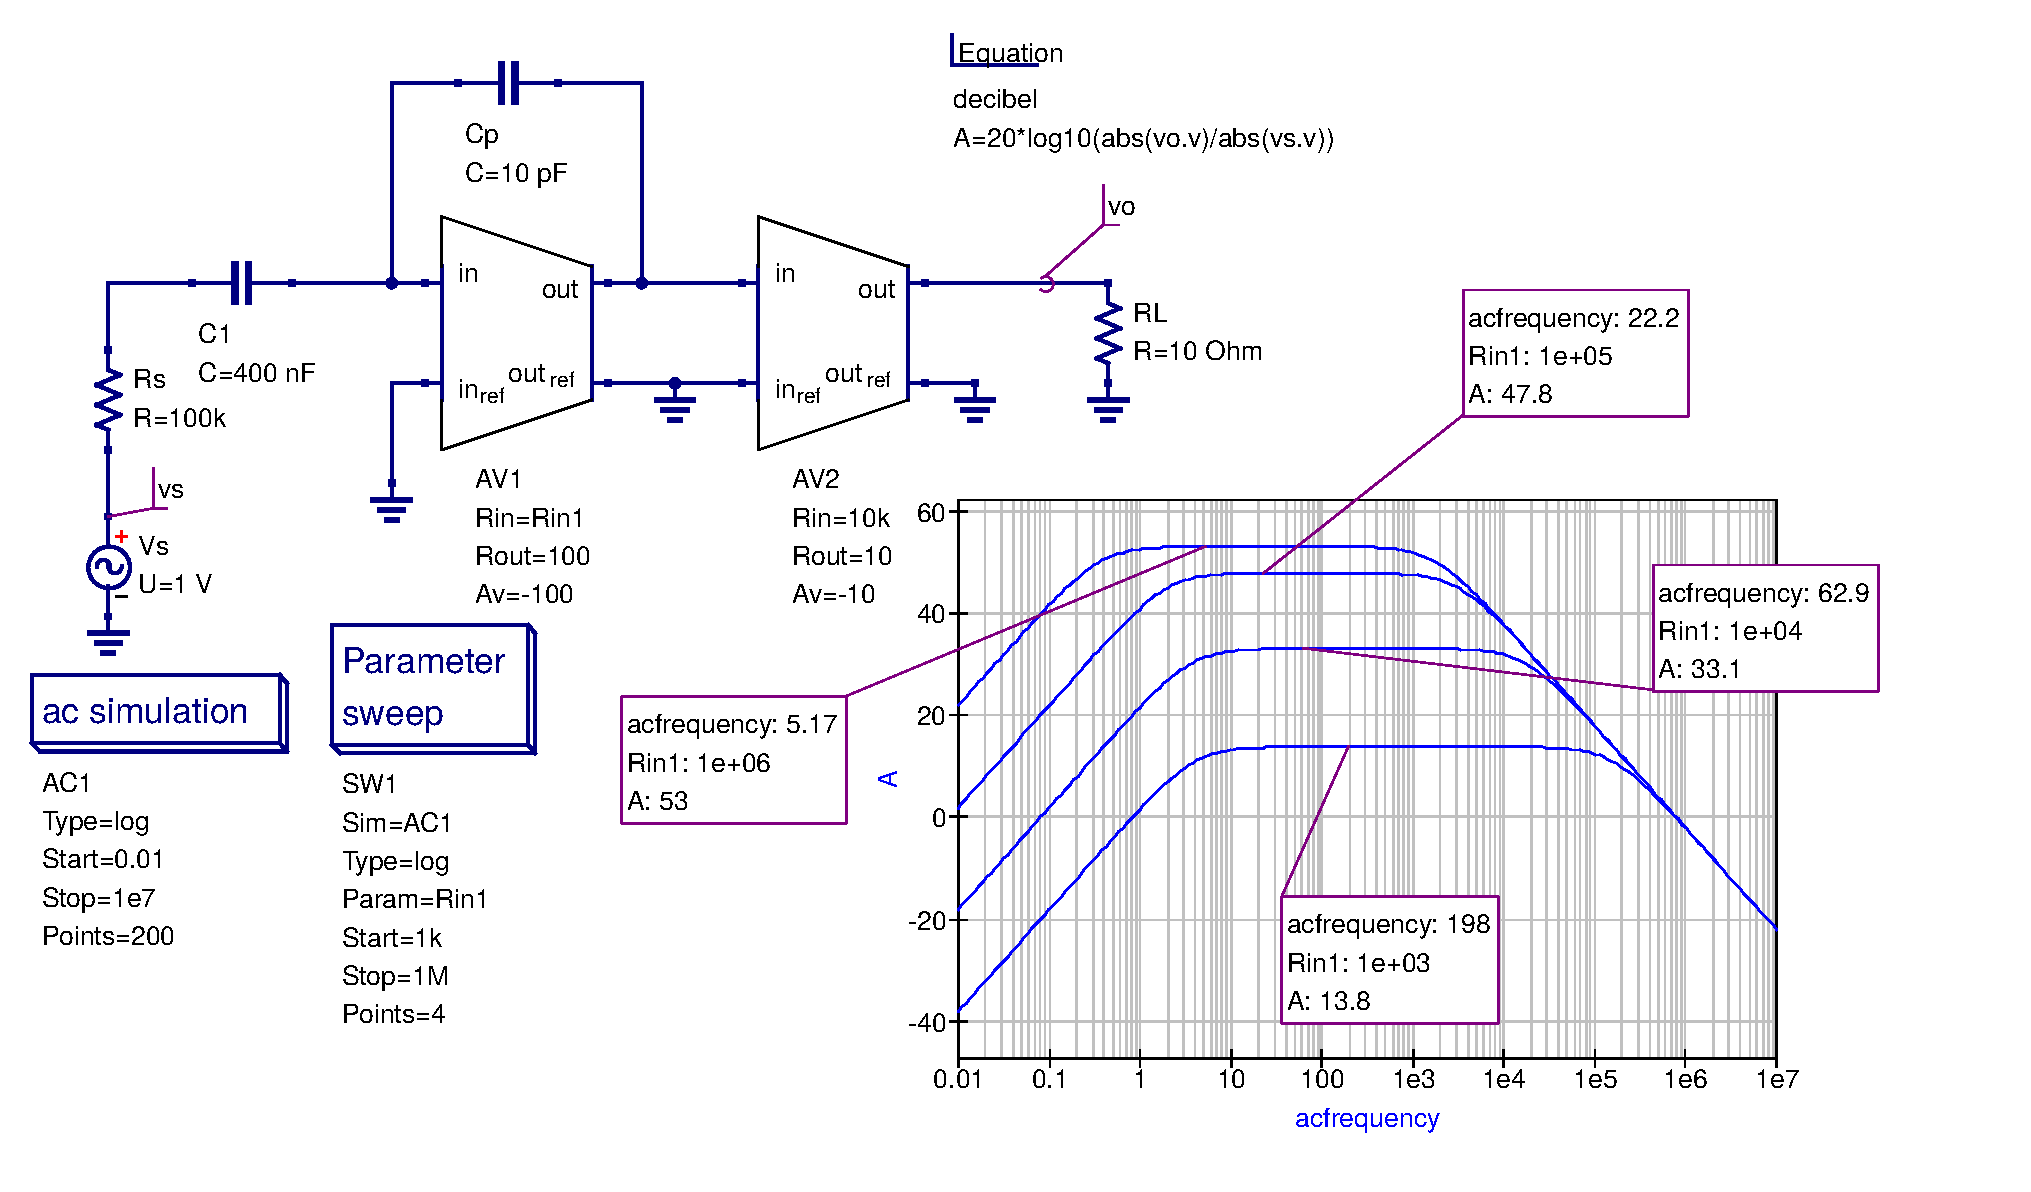
\includegraphics[angle=90, height=0.95\textheight]{ampliBW}
\end{center}
\vfill\eject

% \end{document}

\tutend
